%!TEX root = ../nwoods_thesis.tex

\chapter{Analysis Strategy}

\section{Background Estimation}
Reducible backgrounds for four-lepton events typically have two prompt leptons and two other objects---typically jet fragments, sometimes photons---which are misidentified as prompt leptons.
The largest source of background contamination is from evens in which a {\PZ} boson is produced in association with a photon and a jet, a leptonically-decaying $\PW$ boson and a jet, or two jets.
There is also a contribution from {\TTbar} events in which both top quarks decay to a lepton, a neutrino, and a {\Pqb}~quark jet.
For simplicity, the two sets of processes are not treated separately in what follows, and are collectively labeled ``$\PZ+\PX$'' events.

The contributions of the reducible backgrounds to the selected four-lepton signal samples are evaluated using the tight-to-loose ``fake rates'' method, described more fully in Ref.~\cite{Chatrchyan:2013mxa}.
In this procedure, the likelihood of a nonprompt (``fake'') object to be misidentified as a prompt lepton is estimated and applied to control regions enriched with $\PZ+\PX$ events to estimate their contribution to the signal region.
The lepton misidentification rate $f_\ell\left(\pt^\ell, \eta^\ell\right)$ is measured from a sample of $\PZ + \ell_\text{fake}$ events, where the {\PZ} candidate is selected as in the signal region but with $\left| m_{\ell\ell} - m_\PZ \right| < 10\GeV$, and the $\ell_\text{fake}$ object is a lepton candidate that passes relaxed ID requirements as defined in Section~\ref{sec:looseID}, with no isolation or tight ID requirements applied.
Events with three prompt leptons can contaminate this control region, because the {non-\PZ} lepton is assumed fake.
To avoid the resulting bias in the misidentification rate, the contribution of $\WZ \to 3\ell\nu$ to the $\PZ+\ell_\text{fake}$ sample is estimated from a simulated sample and subtracted.

The misidentification rate is defined as the fraction of $\ell_\text{fake}$ candidates which pass full lepton identification and isolation critera, in bins of $\pt$ and $\eta$.
One should note that this is not a probability in the usual sense, and there is not a simple physical interpretation of these misidentification rates.
Figure~\ref{fig:fakerates} shows the misidentification rates for electrons and muons separately as a function of {\pt} and $\eta$.

\begin{figure}[htbp]
  \begin{center}
    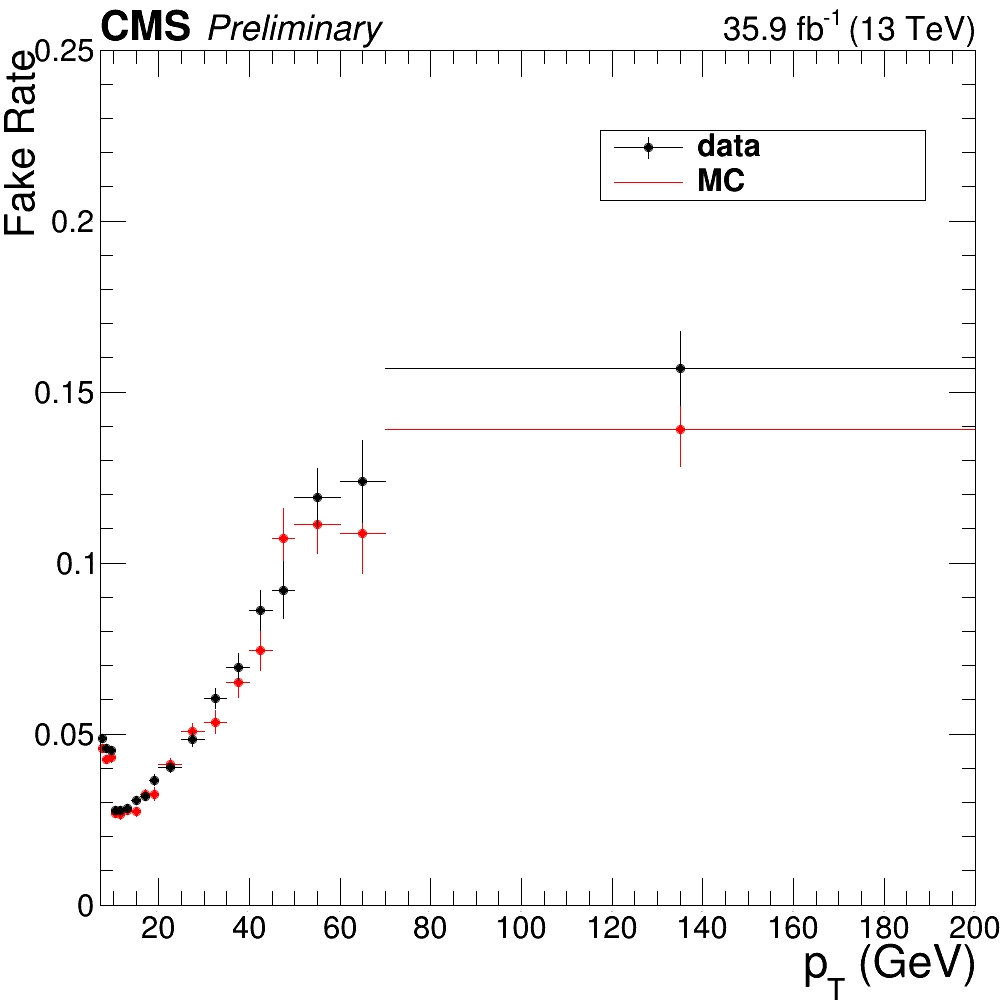
\includegraphics[width=0.35\textwidth]{methods/eFakeRate_pt.png}
    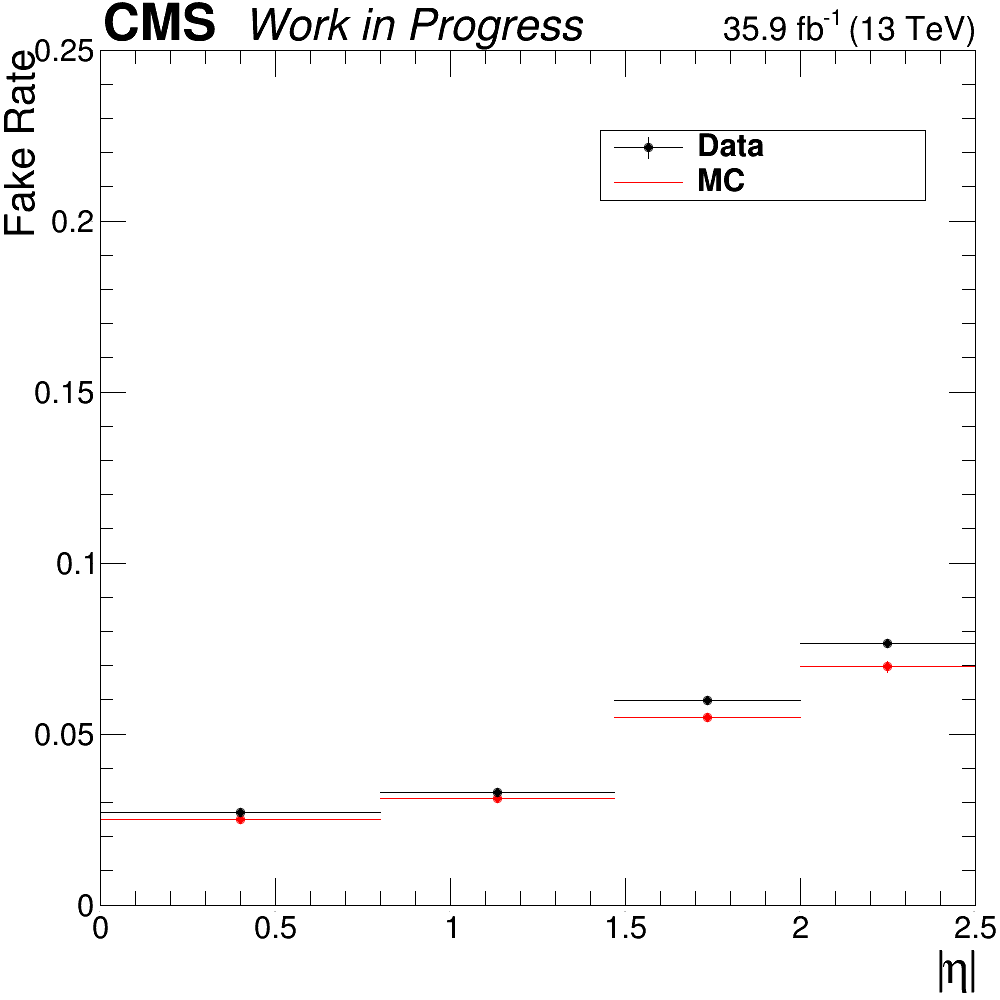
\includegraphics[width=0.35\textwidth]{methods/eFakeRate_eta.png} \\
    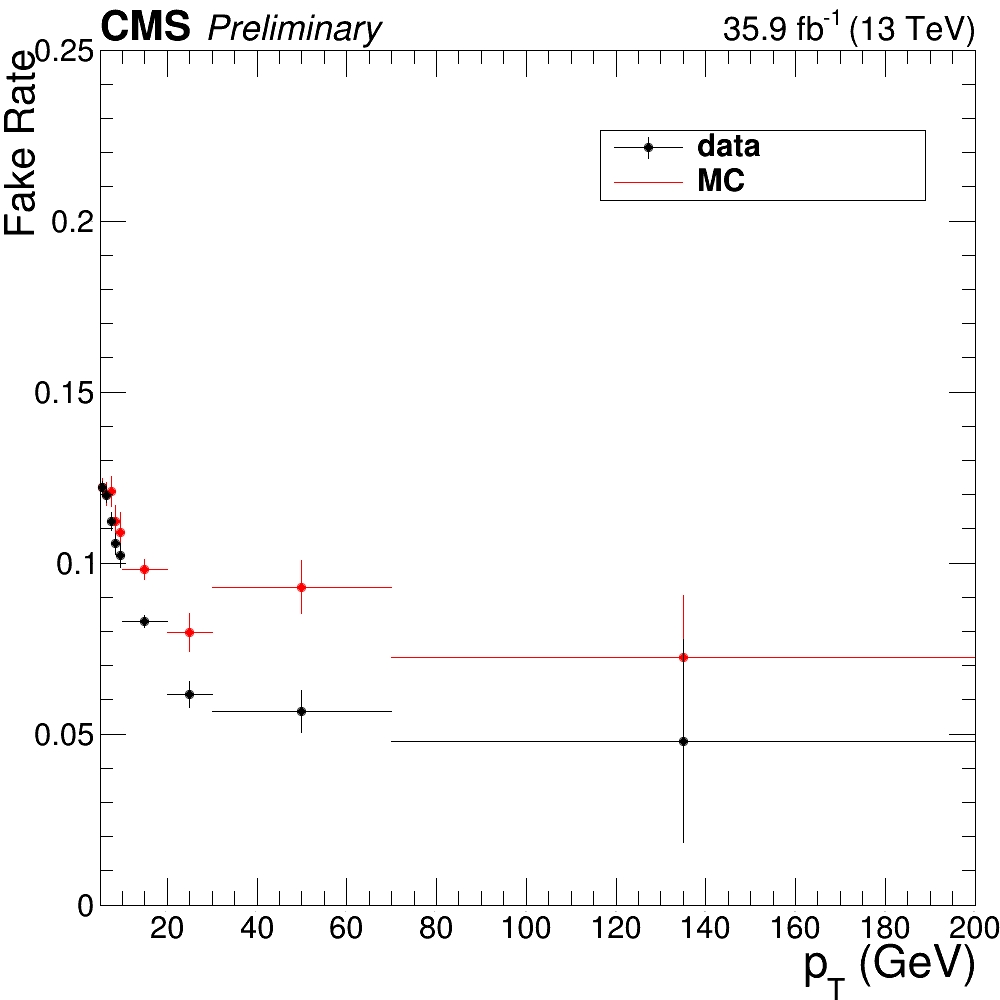
\includegraphics[width=0.35\textwidth]{methods/mFakeRate_pt.png}
    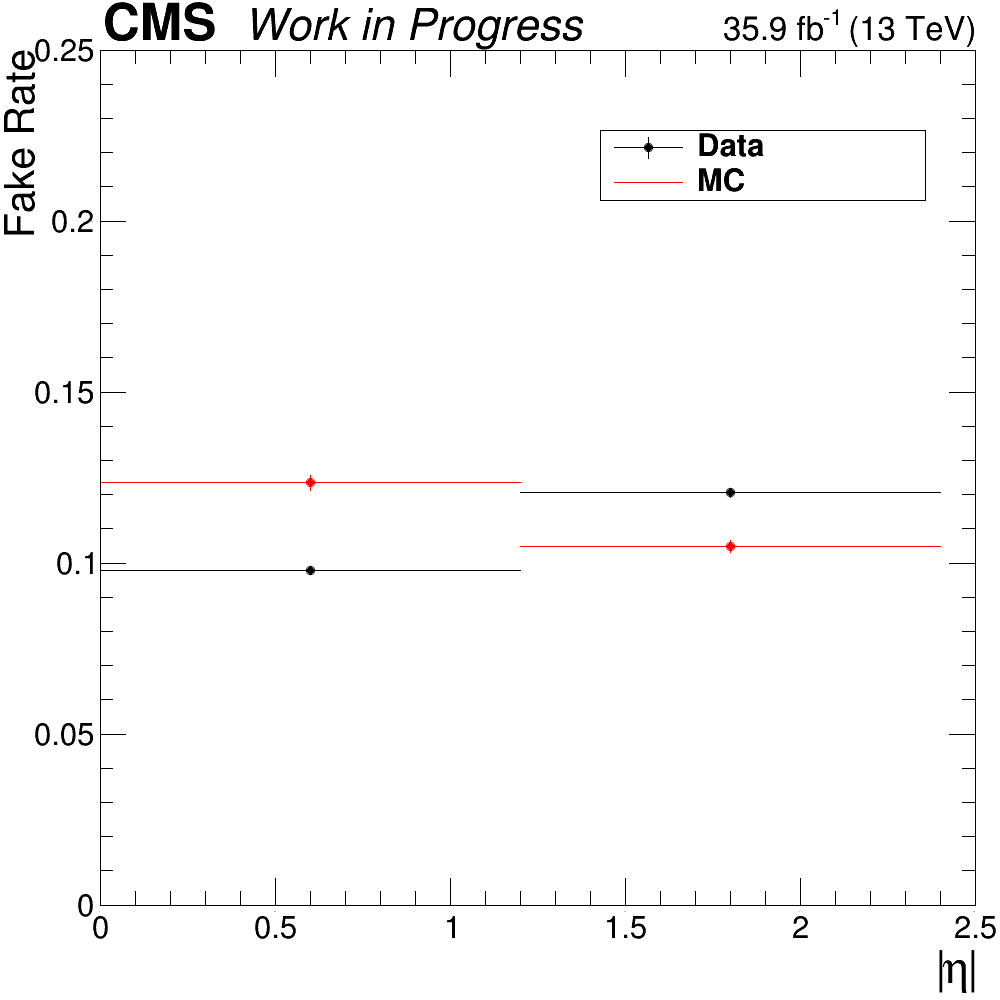
\includegraphics[width=0.35\textwidth]{methods/mFakeRate_eta.png}
    \caption[Misidentification rates for electrons and muons]{
      Fake rate for electrons~(top) and muons~(bottom) as a function of $\pt$~(left) and $\eta$~(right).
      }\label{fig:fakerates}
  \end{center}
\end{figure}

To estimate the total reducible background yield, the misidentification rates are applied to two $\PZ+\PX$ enriched control samples, each containing a {\PZ}~boson candidate passing all signal region requirements plus two more lepton candidates which pass the relaxed identification criteria and would make a second passing {\PZ} boson candidate except that one or both fail the full identification or isolation criteria.
The sample with one failing lepton, called the ``3P1F'' sample for ``3 prompt 1 fake,'' covers the contribution from {\WZ} events, while the sample with both leptons in the second {\PZ} boson failing (``2P2F'') covers $\PZ+\text{jets}$ and {\TTbar} events.
Both have the contribution from {\ZZ} events in which one or two prompt leptons fail identification or isolation criteria removed based on simulated samples.
The fake object transfer factor
\begin{equation}
  F_\ell\left(\pt^\ell,\eta^\ell\right) = \frac{f_\ell\left(\pt^\ell, \eta^\ell\right)}{1 - f_\ell\left(\pt^\ell, \eta^\ell\right)}
\end{equation}
is the ratio of nonprompt objects passing the relaxed and full selection criteria, and thus serves as an extrapolation factor between control sample yields and signal sample yields.

The total reducible background yield is thus
\begin{equation}\label{eq:bkgYield}
  N_\text{bkg} = \sum_{\ell \in \text{3P1F}} F_\ell\left(\pt^\ell,\eta^\ell\right) - \sum_{\ell_1,\ell_2 \in 2P2F} F_{\ell_1}\left(\pt^{\ell_1},\eta^{\ell_1}\right)F_{\ell_2}\left(\pt^{\ell_2},\eta^{\ell_2}\right),
\end{equation}
where subtraction of signal contamination is implicit.
The minus sign in Eq.~\ref{eq:bkgYield} prevents double-counting of $\PZ+2\text{jets}$ events in which one jet fragment is misidentified.

There are also irreducible background contributions from {\TTZ} and {\WWZ} events, which can have four prompt leptons.
Expected yields for these processes are taken from simulation.



\section{Systematic Uncertainties}

Systematic uncertainties for trigger efficiency are taken to be the difference between trigger efficiencies in data and in simulated events, found to be around 2\% of the final event yield.
Because leptons in $\PZ \to 4\ell$ events generally have lower $\pt$, the uncertainty increases to 4\% for $\PZ \to 4\Pe$ events.
In both data and simulated events, trigger efficiencies are found with a tag-and-probe technique~\cite{CMS:2011aa}, performed on four-lepton events.

The lepton identification and isolation efficiencies in simulation are corrected with scaling factors derived with the tag-and-probe method, performed on a sample of $\PZ \to \ell^+\ell^-$ events.
To find the uncertainties associated with these corrections, the total yield is recomputed with the scaling factors varied up and down by the tag-and-probe uncertainties, treating all bins as correlated.
The uncertainties in the $\ZZ \to 4\ell$ yield associated with the tag-and-probe results are found to be 6\% in the $4\Pe$ final state, 3\% in the $2\Pe2\Pm$ final state, and 2\% in the $4\Pm$ final state.
Leptons in $\PZ \to 4\ell$ events tend to have lower {\pt}, and the tag-and-probe samples for low-$\pt$ leptons are smaller and more contaminated with nonprompt objects, so the uncertainties are larger; they are found to be 10\%, 6\%, and 7\% for the $4\Pe$, $2\Pe\Pm$, and $4\Pm$ final states, respectively.

The uncertainty on the LHC integrated luminosity of the data sample is 2.5\%.

The uncertainty on lepton fake rates is taken to be 40\%, which includes both statistical uncertainty and systematic uncertainties associated with the loosened lepton selections used and the differences in the underlying physics processes between events in the $3\ell$ and $4\ell$ control samples.
Statistical uncertainties arising from the limited size of the $\PZ+\PX$ control samples is also included as a systematic uncertainty on the background yield.
The total uncertainty on the background yield varies by channel but is below 1\% of the expected total yield.

Uncertainties due to the effect of QCD scale on the $\ZZ \to 4\ell$ acceptance are evaluated with {\POWHEG} and {\MCFM}, by varying the QCD scales up and down by a factor of two with respect to the default $\mu_R = \mu_F = m_{\ZZ}$.
Parametric  uncertainties (PDF$+ \alpha_s$) are evaluated according to the \textsc{pdf4lhc} prescription in the acceptance calculation~\cite{Butterworth:2015oua}, and with \textsc{nnpdf3.0} in the cross section calculations.
An additional theoretical uncertainty arises from scaling the $\Pq\Paq \to \ZZ$ and $\Pg\Pg \to \ZZ$ simulated samples to their NNLO and NLO predicted cross sections, respectively.
The corresponding change in the acceptance, 1.1\%, is added to the previous theoretical errors in quadrature.

Systematic uncertainties on expected signal yield are summarized in Table~\ref{tab:systematics}.
To obtain uncertainties in computed quantities such as cross sections, the inputs are varied separately for each source and the calculation is fully redone.
For differential cross section and other shape uncertainties, the variations across bins are taken to be fully correlated for each uncertainty source.
Lepton and jet momentum scale and resolution uncertainties are taken to be trivial for the overall yield, but they are considered among the shape uncertainties.

\begin{table}[htbp]
  \centering
  \caption[Systematic uncertainties on the total yield]{
    The contributions of each source of signal systematic uncertainty in the total yields.
    The integrated luminosity uncertainty and the PDF and scale     uncertainties are considered separately.
    All other uncertainties are added in quadrature into a single systematic uncertainty.
    Uncertainties that vary by decay channel are listed as a range.
  }\label{tab:systematics}
  \begin{tabular}{lcc}
    \toprule
    Uncertainty               & $\PZ  \to  4\ell$ & $\ZZ  \to  4\ell$  \\
    \midrule
    Lepton efficiency         & 6--10\%           & 2--6\%             \\
    Trigger efficiency        & 2--4\%            & 2\%                \\
    MC statistics             & 1--2\%            & 0.5\%              \\
    Background                & 0.6--1.3\%        & 0.5--1\%           \\
    Pileup                    & 1--2\%            & 1\%                \\
    \midrule
    PDF                       & 1\%               & 1\%                \\
    QCD Scales                & 1\%               & 1\%                \\
    \midrule
    Integrated luminosity     & 2.5\%             & 2.5\%              \\
    \bottomrule
  \end{tabular}
\end{table}



\section{Fiducial and Total Cross Section Calculation}

Inclusive cross section measurements can be treated as simple binned counting experiments, where the bins are the three decay channels ($4\Pe, 2\Pe2\Pm$, and $4\Pm$).
If $\nu_i$ events are expected in bin $i$, the probability of observing $n_i$ events is given by the Poisson distribution,
\begin{equation}
  f\left(n_i; \nu_i\right) = e^{-\nu_i}\frac{\nu_i^{n_i}}{n_i !}.
\end{equation}

\subsection{Signal Strength Extraction}
Fitting


\subsection{\texorpdfstring{$\mathrm{Z} \to 4\ell$}{Z to 4l} Branching Fraction}
It is tiny



\section{Differential Cross Sections}

\subsection{Unfolding}
IT'S FREQUENTIST\@!


\subsection{Propagation of Systematic Uncertainties}
A small pain



\section{VBS Signal Extraction}
BDTs and other hip things



\section{Anomalous Gauge Coupling Searches}
